\documentclass{article}
\usepackage{blindtext}
\usepackage[T1]{fontenc}
\usepackage[utf8]{inputenc}
\usepackage[margin=0.75in]{geometry}
\usepackage{url}
\usepackage{hyperref}
\usepackage{amsfonts}
\usepackage{graphicx}

\begin{document}

\begin{center}

%\LARGE{\textbf{Research Proposal}} \\
%\vspace{1em}
\Large{15-418 Final Project Proposal} \\
\vspace{1em}
\normalsize\textbf{Manish Nagireddy (mnagired) and Ziad Khattab (zkhattab)} \\
\vspace{1em}

\end{center}

\section*{Title}

An Exploration of Parallelism in Neural Networks

\section*{Summary}

For our 15-418 final project, we are looking into potential axes of parallelism that exist within neural networks. We will be implementing neural networks in both \texttt{C++} (via \texttt{OpenMP}) and \texttt{Python} (via \texttt{PyTorch} and potentially \texttt{mpi4py}, an MPI package for Python) and measuring their performance on CPUs as well as GPUs.

\section*{Background}

In recent years, we have seen the rapid increase of neural networks within the landscape of artificial intelligence, and more broadly within algorithmic decision making. However, because of the large size of these models (given by the number of parameters) as well as the large size of the data used to train them, performance of these so-called deep learning paradigms can be suboptimal without specific attention to parallelism. \\

Broadly, from the perspective of a neural network, there are two dimensions to parallelize: the data and the model.

\begin{enumerate}
  \item \textbf{Data Parallelism:}
  \begin{itemize}
    \item given $X$ machines/cores, split the data into $X$ partitions and use the \textit{same} model to train each partition of the data on a different device in parallel. Then, combine the resultant model weights from each partition
    \item Note that this is model agnostic because it relies only on the data
  \end{itemize}
  \item \textbf{Model Parallelism:}
  \begin{itemize}
    \item splitting the model into various partitions and assigning them to different machines.
    \item NOTE: there are dependencies that are specific to specific model architectures, and so model parallelism is not really ``parallel" because we are actually just assigning consecutive layers of a model to different devices. Some have referred to this as \textit{model serialization}\footnote{\href{https://leimao.github.io/blog/Data-Parallelism-vs-Model-Paralelism/}{Data Parallelism VS Model Parallelism in Distributed Deep Learning Training - Lei Mao's Log Book}}
    \item commonly used when the model is too large to fit on a single device
  \end{itemize}
\end{enumerate}

Refer to the figure\footnote{\href{https://xiandong79.github.io/Intro-Distributed-Deep-Learning}{Link to Figure Citation}} below for an illustration of data parallelism and model parallelism.

\begin{figure}[h]
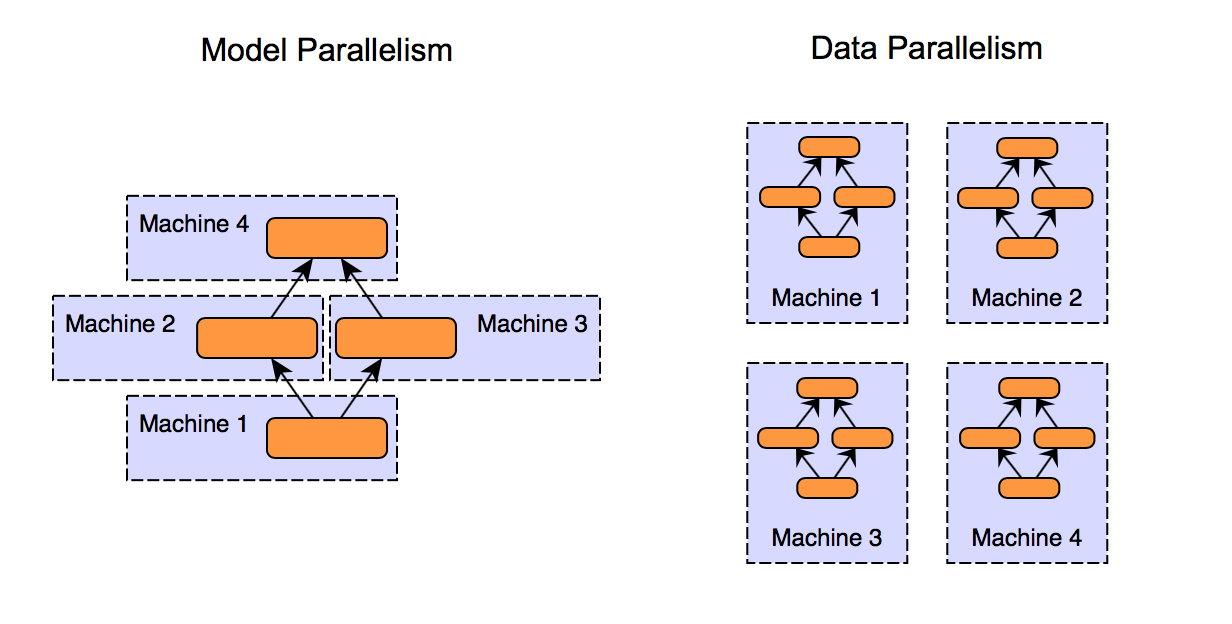
\includegraphics[scale = 0.45]{background}
\centering
\end{figure}

\section*{The Challenge}

The main challenge stems from the fact that there exist a lot of dependencies when working with a neural network. At the lowest, implementation-detail level, we know that different architectures have different structures and therefore different dependencies between layers (e.g. between input and hidden layers). But we also know that the choice of hyperparameters (e.g. learning rate) and optimizers (e.g. Stochastic Gradient Descent or SGD, Adam, AdaGrad, etc.) heavily influence model convergence time as well as model performance. In addition, we have that the choice of dataset is also significant (and related) to the class of models we use. Finally, we are limited by the choice of compute power, in the sense that we can only measure performance on machines with fixed number of CPU cores as well as fixed numbers of GPUs.\\

Given that we want to focus on parallelism, we do \textit{not} want to get caught up in trying out different models on different datasets with different parameters. Thus, we will fix our dataset to be the widely well-known benchmark MNIST\footnote{\href{http://yann.lecun.com/exdb/mnist/}{Link to MNIST Data}} dataset. This also restricts us to the problem of image classification, where further restricts the class of neural networks that we will be looking at (e.g. now we can focus on simple feed forward networks and basic convolutional neural networks or CNNs). From background research, this dataset is known to be relatively cheap to train and still have nontrivial results without excessive preprocessing of the input data.\\

Then, we're able to focus the ``unknown" aspects of our project to be the axes of parallelism and their corresponding performance or speedups. Specifically, once we have a baseline performance in a shared memory setting, we can transition and aim to look at the difference between data and model parallelism, as well as the specific differences within data parallelism (e.g. multi core vs single GPU vs multi GPU). \\

To make this more concrete, here is the high level sequence of our project:

\begin{enumerate}
  \item Implement and compare a \texttt{C++} version with a \texttt{C++/OpenMP} of a very basic model to serve as a reference for speedup and performance
  \item Shift to \texttt{Python} and begin comparing both basic and complicated models via data and model parallelism
  \begin{itemize}
    \item For data parallelism: experiment with different batch sizes (explained below)
    \item For model parallelism: experiment with models on multi core vs single GPU vs multi GPU
  \end{itemize}
\end{enumerate}

\section*{Resources}

Given that we want to explore the differences in axes of parallelism, we will try not to spend too much time implementing sequential neural networks from scratch. From the \texttt{C++} standpoint, there exists an abundance of starter code (e.g. [\href{https://github.com/Whiax/NeuralNetworkCpp/tree/master/src/neural}{1},\href{https://github.com/huangzehao/SimpleNeuralNetwork/blob/master/src/neural-net.cpp}{2},\href{https://github.com/arnobastenhof/mnist/tree/master/src}{3}]). For \texttt{Python}, we will rely upon the \texttt{PyTorch} documentation for commonly used neural networks (e.g. standard CNN or basic ResNet). \textit{The main coding portion (in \texttt{C++}) will come from translating a \texttt{C++} implementation of a neural network into an OpenMP version}. \\

Additionally, there is a very interesting article from folks at Google Research\footnote{\href{https://ai.googleblog.com/2019/03/measuring-limits-of-data-parallel.html}{Measuring the Limits of Data Parallel Training for Neural Networks}} which describes the various scaling patterns that they observed during data parallelism. Note that their measurement of data parallelism is directly related to the batch size, which is the number of training data examples utilized in one iteration of training the model. Specifically, they discovered three distinct but related so-called ``scaling-regimes":
\begin{enumerate}
  \item Perfect Scaling: doubling batch size halves number of training steps to reach some target error
  \item Diminishing Returns: fewer decreases to training time with increasing batch size
  \item Maximal Data Parallelism: further increasing batch size beyond this point doesn’t reduce training time
\end{enumerate}

We will attempt to see if this pattern can also be observed with our model and comment on any differences. Note that this will only be possible for the \texttt{Python} models due to the features provided by \texttt{PyTorch}\\

\noindent Finally, regarding the computing resources required for our project, we will use the following:

\begin{itemize}
  \item For Single GPU: we will use AWS EC2 \texttt{g4dn.xlarge} which comes with 1 GPU. One of the team members has around \$45 in credits from a previous deep learning course so we should hopefully not need any more than this
  \item For Multi-GPUs (to be used only in model parallelism): we will use the PSC-Bridges 2 machines which have either 8 or 16 GPUs
  \item For Multi-Core: we will either use the Gates machines for lower core counts, or talk to the professors about getting access to higher core count machines (e.g. 32 or 64 cores).
\end{itemize}

\section*{Goals and Deliverables}

\paragraph{PLAN TO ACHIEVE} A successful project would entail a comparison between data and model parallelism with respect to speedup as well as performance. This would involve having a working implementation of our models in \texttt{C++} with and without \texttt{OpenMP} to be able to comment on performance and speedup in a shared memory setting. Then, we shift to our \texttt{Python} models and have measurements of speedup with respect to both data and model parallelism. For an example of a specific metric we may want to look out for, we will see if we can achieve the result that doubling batch size (so in the data parallel setting) halves the training time.

\paragraph{HOPE TO ACHIEVE} If everything is going very well and we are able to get all of these measurements, we will experiment with also adding a message-passing model (via \texttt{mpi4py} in \texttt{Python}) to our set of models.

\paragraph{75\%} If everything is going slower than intended, then we will pick only one of data or model parallelism to proceed forward with, depedending on what seems more suitable given our resource and time constraints.

\paragraph{Poster Session Demo} Ideally, we would like to be able to run an iteration of our model training and output a classification, across the different model types. Realistically, this may not be feasible given the resources we need (e.g. we may not be able to have a 16 GPU machine on standby) and so we will try to at least show multi-core (via AWS or GHC) at the minimum. We will also definitely show our speedup and performance graphs.

\paragraph{Learning Objectives} Our learning objectives are as follows:

\begin{itemize}
  \item Think about the inherent dependencies within a deep learning pipeline when attempting to implement a neural network via shared memory
  \item Comment on the effectiveness of data and/or model parallelism in the example of a reasonably complex data and model setting
\end{itemize}

\section*{Platform Choice} Given that the majority of this class is focused on \texttt{C++}, we want to be able to use it (along with \texttt{OpenMP}) as a starting point. We also think it would be interesting to see a neural network within the shared memory context. However, after this initial part (ideally before or right up to the milestone report checkpoint), we will fully transition to \texttt{Python}, taking full advantage of the capabilities of \texttt{PyTorch} as a deep learning framework. \\

As for compute resources, we will be using a combination of AWS EC2, PSC-Bridges 2, GHC cluster machines, and potentially other high core machines from professors to be able to satisfy our different requirements.

\section*{Schedule}

\begin{center}
	\begin{tabular}{ |c|c| }
		\hline
		Week & Goals \\
		\hline
		3/21 - 3/28 & Project proposal and start working on \texttt{C++} implementation \\
		\hline
		3/28 - 4/4 & Finish the \texttt{C++} and start translating to \texttt{OpenMP} implementation\\
		\hline
		4/4 - 4/11 & Finish the shared memory implementation + Milestone Report and start data parallelism in \texttt{Python} \\
		\hline
		4/11 - 4/18 & Finish Data Parallelism and start working on Model Parallelism\\
		\hline
		4/18 - 4/25 & Finish Model Parallelism and start collecting performance metrics, potentially also work on \texttt{MPI} version\\
		\hline
		4/25 - 4/29 & Finish Final Report\\
		\hline
	\end{tabular}\\
\end{center}

\end{document}
